\section{}

% Plot all the collected data (displacement vs voltage) for the potentiometer and
% find the correlating function with a function of the form x=aV+b. Report the equation used 
% in the fit of your data. Determine the sensitivity and span.

\subsection{}
% slope	12.672	-1.499	intercept
% r^2	1.000

The plot of displacement over voltage can be found in Fig. \ref{fig:Q1a}. The slope, intercept, and $R^2$ value of the linear regression 
were determined using \texttt{=LINEST()} in Excel. The results can be found in Table \ref{tab:Q1a}.

\begin{table}[h]
    \centering
    \caption{Linear regression of displacement over voltage}
    \label{tab:Q1a}
    \begin{tabular}{ccc}
        \hline
        Slope & Intercept & $R^2$ \\
        (mm/V) & (mm) & \\
        \midrule
        12.67 & -1.50 & 1.00 \\
        \hline
    \end{tabular}
\end{table}

\begin{figure}[h]
    \centering
    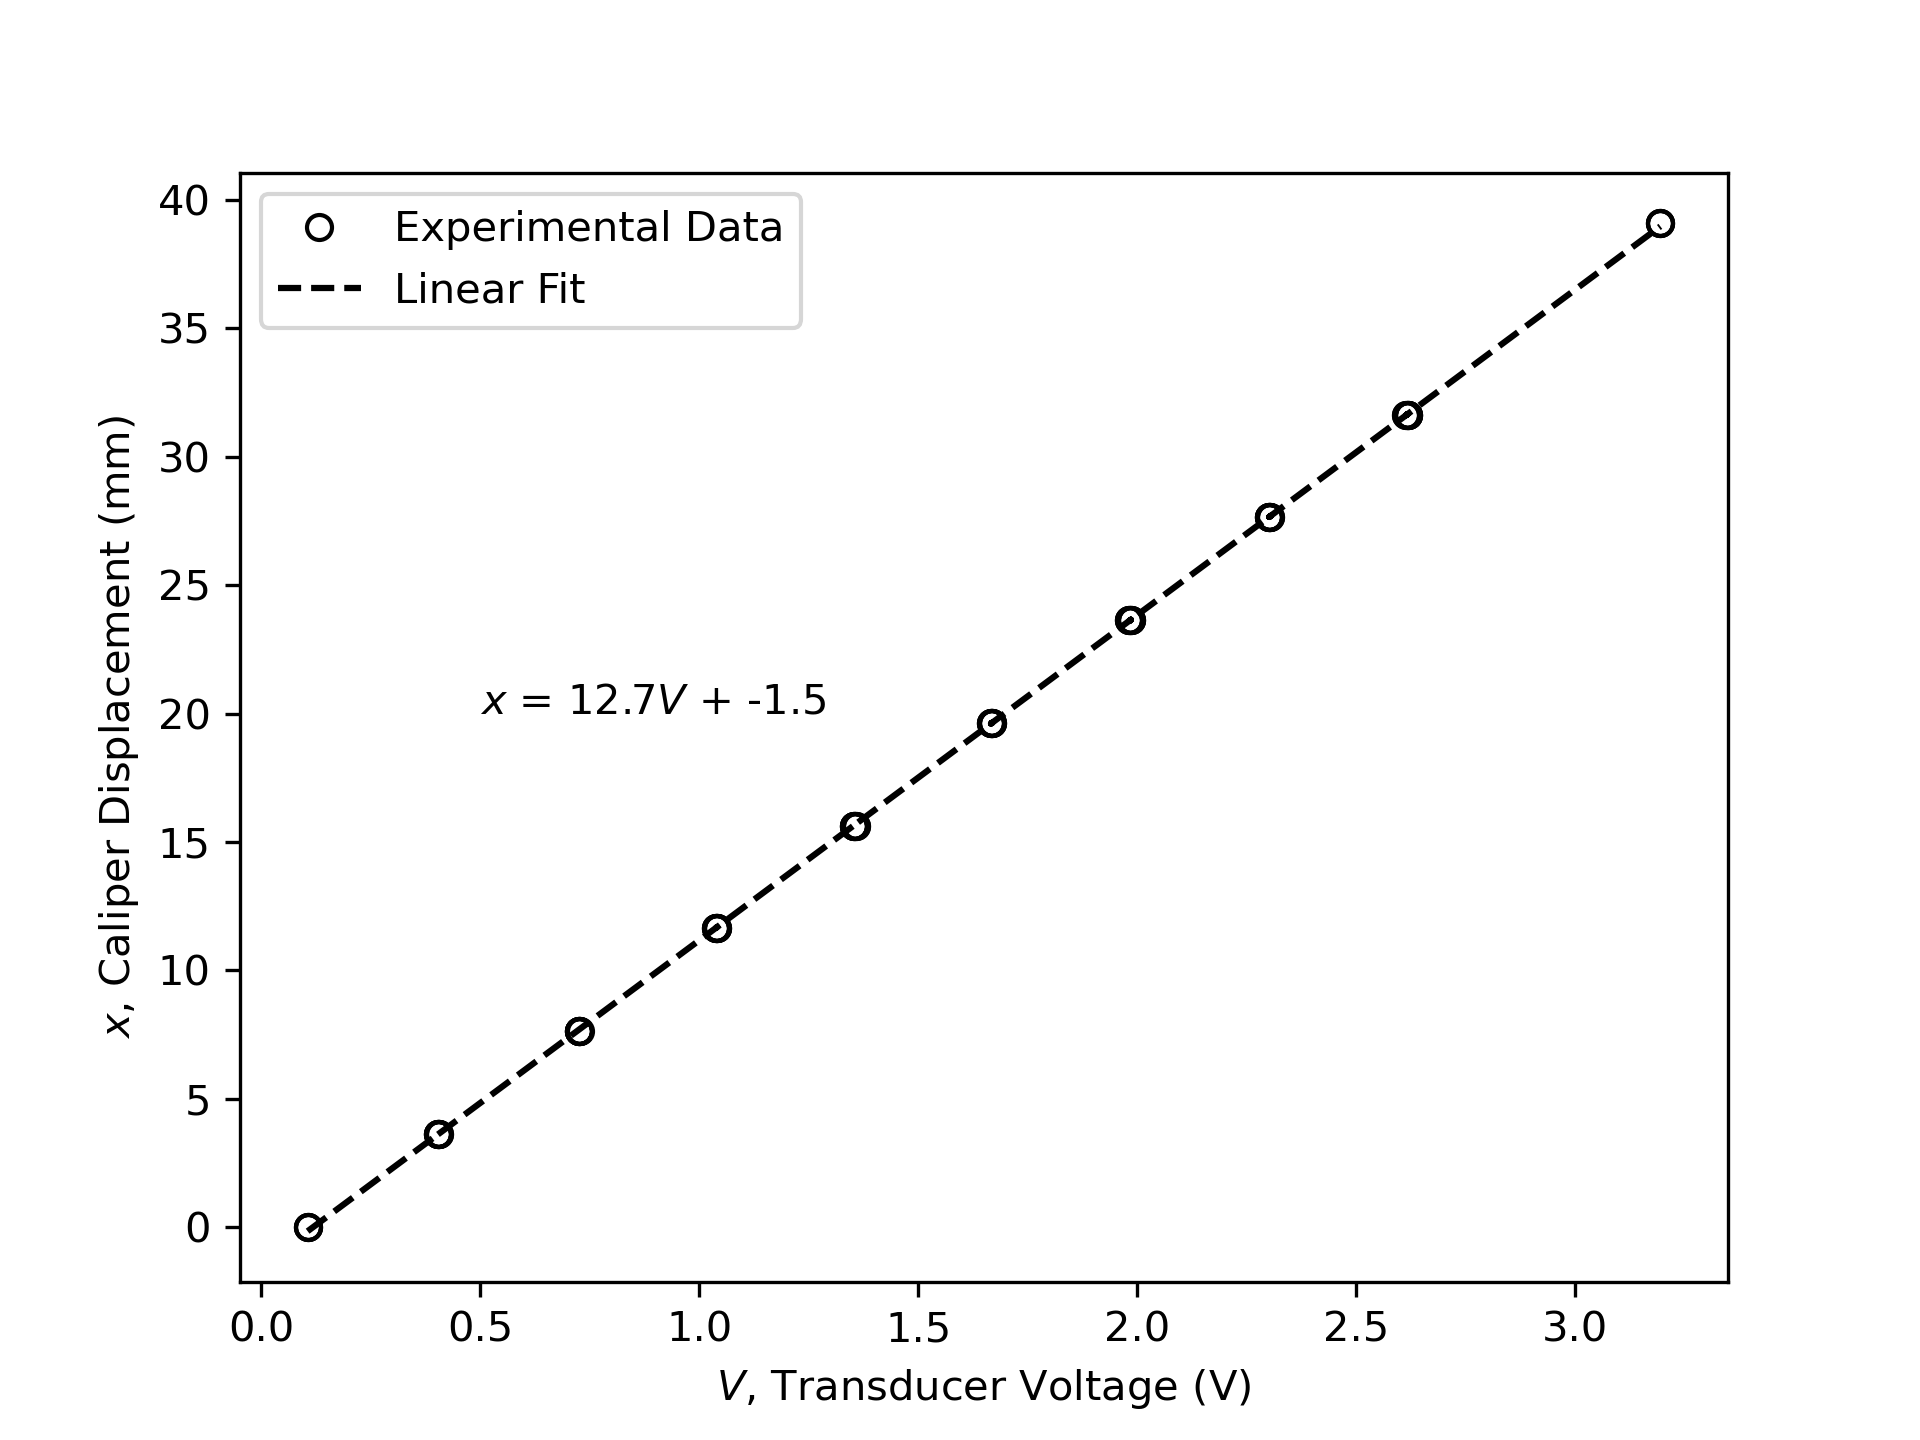
\includegraphics[width=0.8\linewidth]{matplotlib/Q1a.png}
    \caption{Displacement over voltage for the potentiometer}
    \label{fig:Q1a}
\end{figure}


\subsection{}
% b) Make a deviation table, deviation curve, linearity table (independent linearity 
% only), and hysteresis table. Use units of mm.

First, all the voltages were converted to displacements using the linear regression equation found in the previous section. The
displacement table can be found in Appendix \ref{sec:appendix-potentiometer-displacement-table} in Table \ref{tab:appendix-potentiometer-displacement-table}.

The deviation table can be found in Table \ref{tab:Q1b-deviation-table}. The deviation curve can be found in Fig. \ref{fig:Q1b-deviation-curve}.

% deviation table	Up 1	Down 1	Up 2	Down 2	Up 3	Down 3	max dev up	max dev down
% 0.00		-0.155		-0.155		-0.155		0.000
% 3.64	-0.032	-0.032	-0.032	0.006	-0.032	0.006	0.000	0.038
% 7.64	0.049	0.049	0.049	0.049	0.049	0.087	0.000	0.038
% 11.64	0.053	0.053	0.053	0.015	0.015	0.015	0.038	0.038
% 15.64	0.058	0.020	0.020	0.020	0.020	0.058	0.038	0.038
% 19.64	0.012	0.012	-0.026	-0.026	0.012	-0.026	0.038	0.038
% 23.64	0.016	-0.022	0.016	-0.022	0.016	-0.022	0.000	0.000
% 27.64	0.059	0.021	0.021	0.021	0.059	0.021	0.038	0.000
% 31.64	0.025	-0.013	0.025	-0.013	0.025	0.025	0.000	0.038
% 39.10	-0.123		-0.123		-0.123		0.000	

\begin{table}[h]
    \centering
    \caption{Deviation table of potentiometer}
    \label{tab:Q1b-deviation-table}
    \begin{tabular}{cccccc}
        \hline
        Caliper Reading & Up 1 & Down 1 & Up 2 & Down 2 & Up 3 \\
        (mm) & (mm) & (mm) & (mm) & (mm) & (mm) \\
        \midrule
        0.00 & & -0.155 & & -0.155 & \\
        3.64 & 3.608 & 3.608 & 3.608 & 3.646 & 3.608 \\
        7.64 & 7.689 & 7.689 & 7.689 & 7.689 & 7.727 \\
        11.64 & 11.693 & 11.693 & 11.693 & 11.655 & 11.655 \\
        15.64 & 15.698 & 15.660 & 15.660 & 15.660 & 15.660 \\
        19.64 & 19.652 & 19.652 & 19.614 & 19.614 & 19.652 \\
        23.64 & 23.656 & 23.618 & 23.656 & 23.618 & 23.656 \\
        27.64 & 27.699 & 27.661 & 27.661 & 27.661 & 27.699 \\
        31.64 & 31.665 & 31.627 & 31.665 & 31.627 & 31.665 \\
        39.10 & 38.977 & & 38.977 & & 38.977 \\
        \hline
    \end{tabular}
\end{table}

\begin{figure}[h]
    \centering
    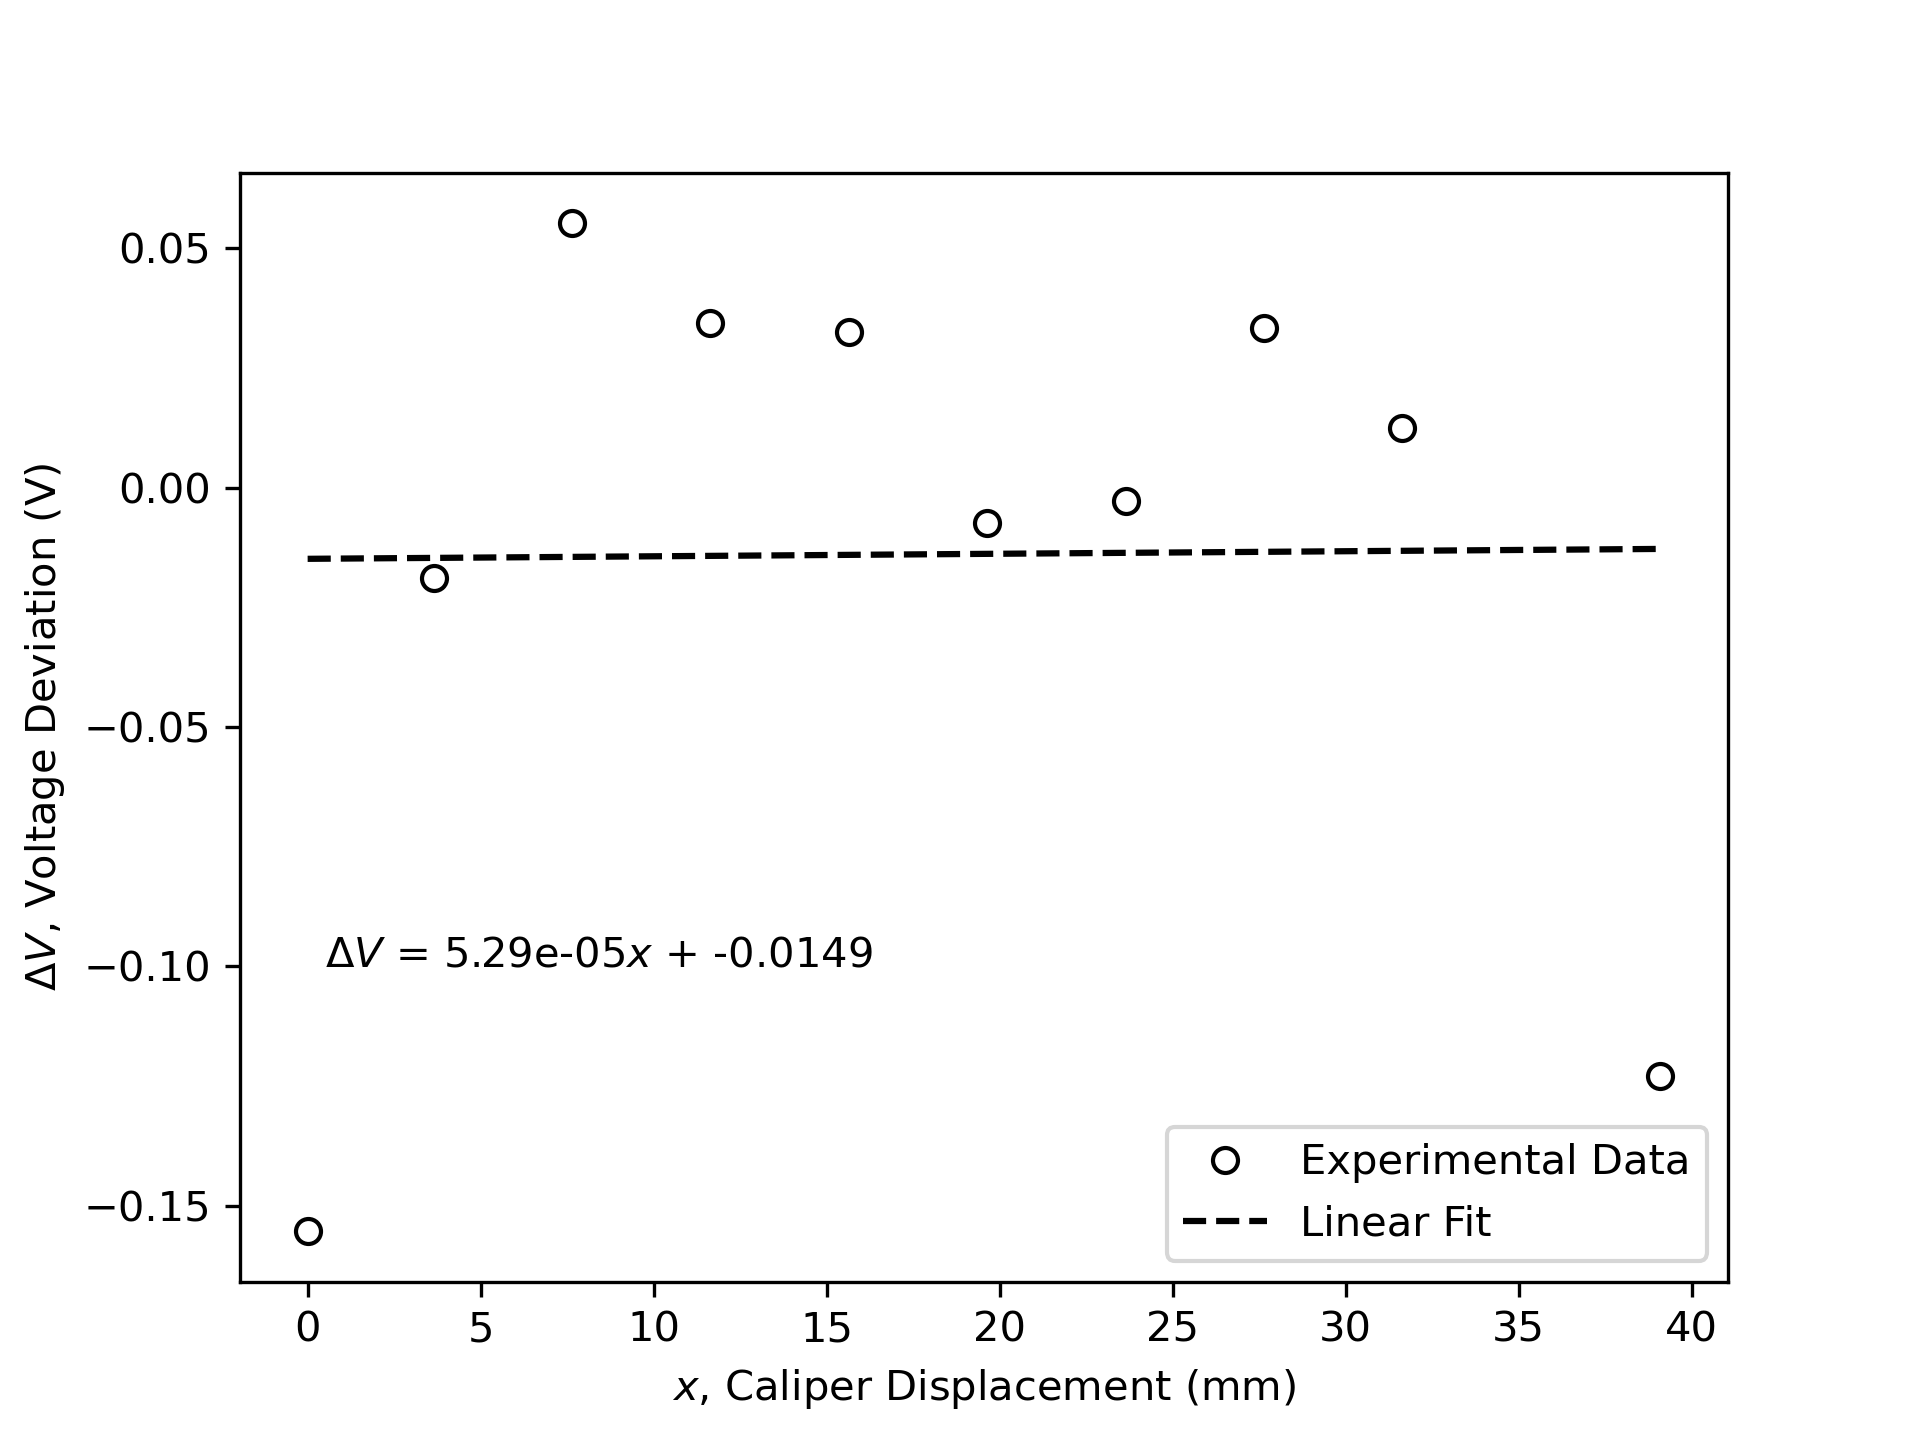
\includegraphics[width=0.8\linewidth]{matplotlib/Q1b.png}
    \caption{Deviation curve of potentiometer with respect to displacement (independent linearity)}
    \label{fig:Q1b-deviation-curve}
\end{figure}